\ccUserChapter{2D Conforming Triangulations and Meshes}
\label{user_chapter_2D_Meshes}

\ccChapterAuthor{Laurent Rineau}

\inout{Mesh_2/PkgDescription}

\minitoc

This package implements Shewchuk's algorithm \cite{s-mgdsa-00} to construct
conforming triangulations and 2D meshes. Conforming triangulations will be
described in Section~\ref{sec:Mesh_2_conforming_triangulation} and
meshes in Section~\ref{sec:Mesh_2_meshes}.

\section{Conforming Triangulations}
\label{sec:Mesh_2_conforming_triangulation}

\subsection{Definitions}
\label{sec:Mesh_2_conforming_definitions}

A triangulation is a \emph{Delaunay triangulation} if the circumscribing
circle of any facet of the triangulation contains no vertex in its
interior. A \emph{constrained} Delaunay triangulation is a constrained
triangulation which is a much Delaunay as possible. The circumscribing
circle of any facet of a constrained Delaunay triangulation contains in its
interior no data point \emph{visible} from the facet.

An edge is said to be a \emph{Delaunay edge} if it is inscribed in an empty
circle (containing no data point in its interior). It is said to be a
\emph{Gabriel edge} if its diametrical circle is empty.

A constrained Delaunay triangulation is said to be a \emph{conforming
  Delaunay triangulation} if every constrained edge is a Delaunay edge.
Because any edge in a constrained Delaunay triangulation is either a
Delaunay edge or a constrained edge, a conforming Delaunay triangulation is
in fact a Delaunay triangulation. The only difference is that some of the
edges are marked as constrained edges.

A constrained Delaunay triangulation is said to be a \emph{conforming
  Gabriel triangulation} if every constrained edge is a Gabriel edge. The
Gabriel property is stronger than the Delaunay property and each Gabriel
edge is a Delaunay edge. Thus conforming Gabriel triangulations are also
conforming Delaunay triangulations.

Any constrained Delaunay triangulation can be refined into a
conforming Delaunay triangulation or a conforming Gabriel
triangulation by adding vertices, called \emph{Steiner vertices}, on
constrained edges until they are cut into subconstraints small enough
to be Delaunay or Gabriel edges.

\subsection{Building Conforming Triangulations}
\label{sec:Mesh_2_building_conforming}

Constrained Delaunay triangulations can be refined into
conforming triangulations 
by two global functions: \\
\ccc{template<class CDT> void make_conforming_Delaunay_2 (CDT& t)}~and\\
\ccc{template<class CDT> void make_conforming_Gabriel_2 (CDT& t)}. 

In both cases, the template parameter \ccc{CDT} must be instantiated
by a constrained Delaunay triangulation class.  Such a class must be a
model of the concept \ccc{ConstrainedDelaunayTriangulation_2}.

There are some requirements on the geometric traits of the constrained
Delaunay triangulation used to instantiate the parameter \ccc{CDT}.
It has to be a model of the concept
\ccc{ConformingDelaunayTriangulationTraits_2}.

The constrained Delaunay triangulation \ccc{t} is passed by reference
and is refined into a conforming Delaunay triangulation or a
conforming Gabriel triangulation by adding vertices, that is, the
triangulation is modified. If the user needs to keep the original
triangulation, he or she has to make a copy of it.

The algorithm used by \ccc{make_conforming_Delaunay_2} and
\ccc{make_conforming_Gabriel_2} builds internal data that would be
computed twice if the two functions are called consecutively on the same
triangulation. In order to avoid these data to be constructed twice, the
advanced user can use the class \ccc{Triangulation_conformer_2<CDT>} to
refine a constrained Delaunay triangulation into a conforming Delaunay
triangulation and then into a conforming Gabriel triangulation. That class
provides also step by step functions. Those functions insert one point at a
time.

\subsection{Example: Making a Triangulation Conforming Delaunay and Then
  Conforming Gabriel}
\label{sec:Mesh_2_example_making_conforming}

This example inserts several segments into a constrained Delaunay
triangulation, makes it conforming Delaunay, and then conforming
Gabriel. At each step, the number of vertices of the triangulation is
printed.

\ccIncludeExampleCode{Mesh_2/conforming.C}

See figures~\ref{Conform-example-conform},
\ref{Conform-example-conform-Delaunay}
and~\ref{Conform-example-conform-Gabriel}.

\begin{figure}[htbp]
\begin{ccTexOnly}
\begin{center}
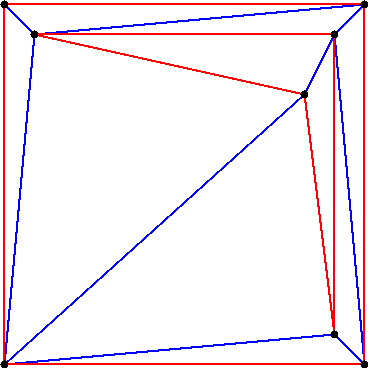
\includegraphics[width=8cm]{Mesh_2/example-conform}
\end{center}
\end{ccTexOnly}
\caption{Initial triangulation.}
\label{Conform-example-conform}

\begin{ccHtmlOnly}
<center>
<img border=0 src="./example-conform.png"
     align=center title="Initial triangulation.">
</center>
\end{ccHtmlOnly}
\end{figure}

\begin{figure}[htbp]
\begin{ccTexOnly}
\begin{center}
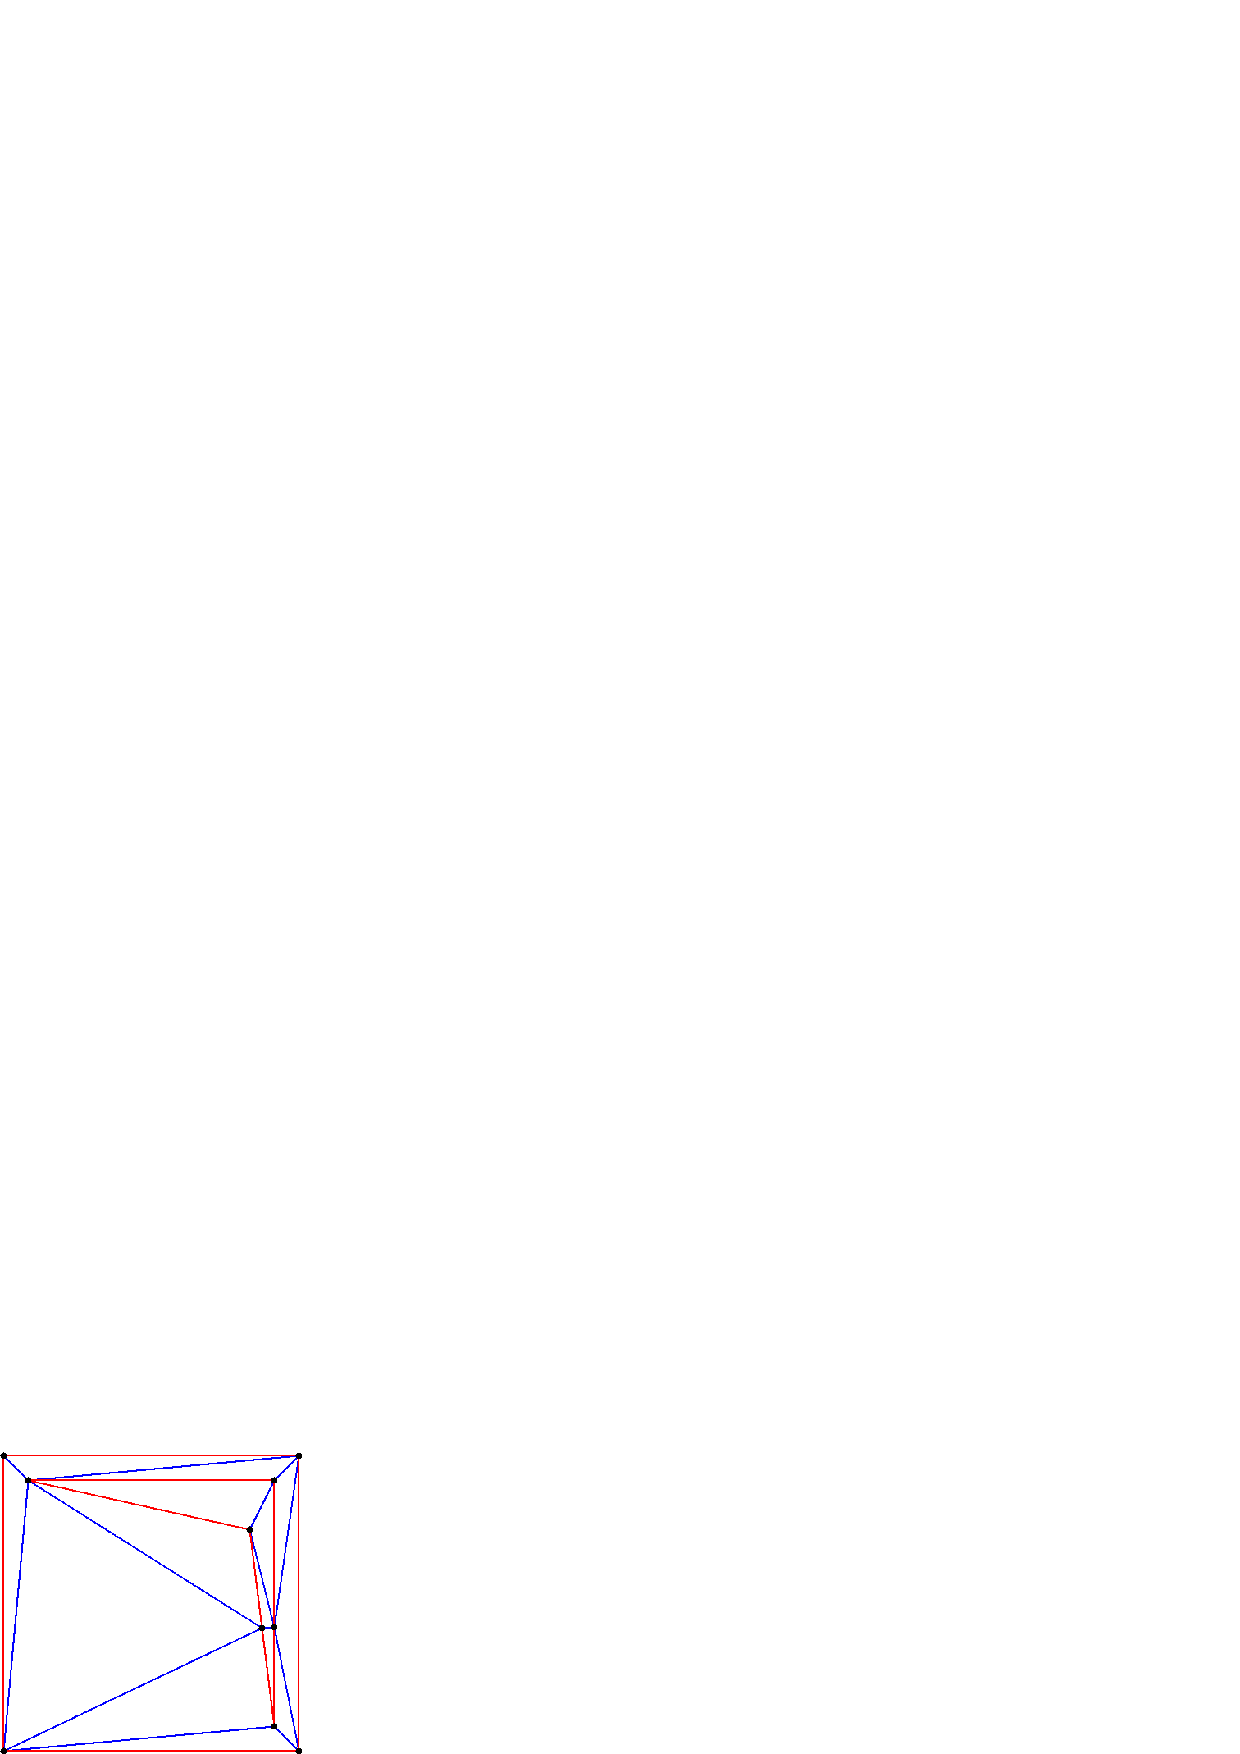
\includegraphics[width=8cm]{Mesh_2/example-conform-Delaunay}
\end{center}
\end{ccTexOnly}
\caption{The corresponding conforming Delaunay triangulation.}
\label{Conform-example-conform-Delaunay}

\begin{ccHtmlOnly}
<center>
<img border=0 src="./example-conform-Delaunay.png"
     align=center title="The corresponding conforming Delaunay triangulation.">
</center>
\end{ccHtmlOnly}
\end{figure}

\begin{figure}[htbp]
\begin{ccTexOnly}
\begin{center}
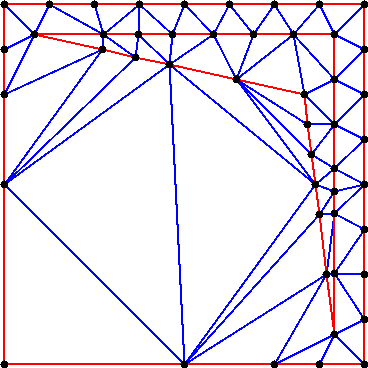
\includegraphics[width=8cm]{Mesh_2/example-conform-Gabriel}
\end{center}
\end{ccTexOnly}
\caption{The corresponding conforming Gabriel triangulation.}
\label{Conform-example-conform-Gabriel}

\begin{ccHtmlOnly}
<center>
<img border=0 src="./example-conform-Gabriel.png"
     align=center title="The corresponding conforming Gabriel triangulation.">
</center>
\end{ccHtmlOnly}
\end{figure}

\section{Meshes}
\label{sec:Mesh_2_meshes}


\subsection{Definitions}
\label{sec:Mesh_2_meshes_definition}

A mesh is a partition of a given region into simplices whose shapes
and sizes satisfy several criteria.

The domain is the region that the user wants to mesh. It has to be
  a bounded region of the plane. The domain is defined by a \emph{planar
  straight line graph}, {\sc Pslg} for short, which is a set of segments
  such that two segments in the set are either disjoint or share an
  endpoint. The segments of the {\sc Pslg} are constraints that will be
  represented by a union of edges in the mesh. The {\sc Pslg} can also
  contain isolated points that will appear as vertices of the mesh.

The segments of the {\sc Pslg} are either segments of the
boundary or internals constraints. The segments of the {\sc Pslg} have to
cover the boundary of the domain.

The {\sc Pslg} divides the plane into several connected components. By
default, the domain is the union of the bounded connected components. The
user can override this default by providing a set of seed points. Either
seed points mark components to be meshed or they mark components not to be
meshed (holes).

See figures~\ref{Domain} and~\ref{Domain-mesh} for an example of a domain
defined without using seed points, and a possible mesh of it. See
figure~\ref{Domain-seeds} for another domain defined with the same {\sc
  Pslg} and two seed points. The two seed points define two holes in the
domain. In the corresponding mesh (figure~\ref{Domain-seeds-mesh}), these
two holes are triangulated but not meshed.

\begin{figure}[htbp]
\begin{ccTexOnly}
\begin{center}
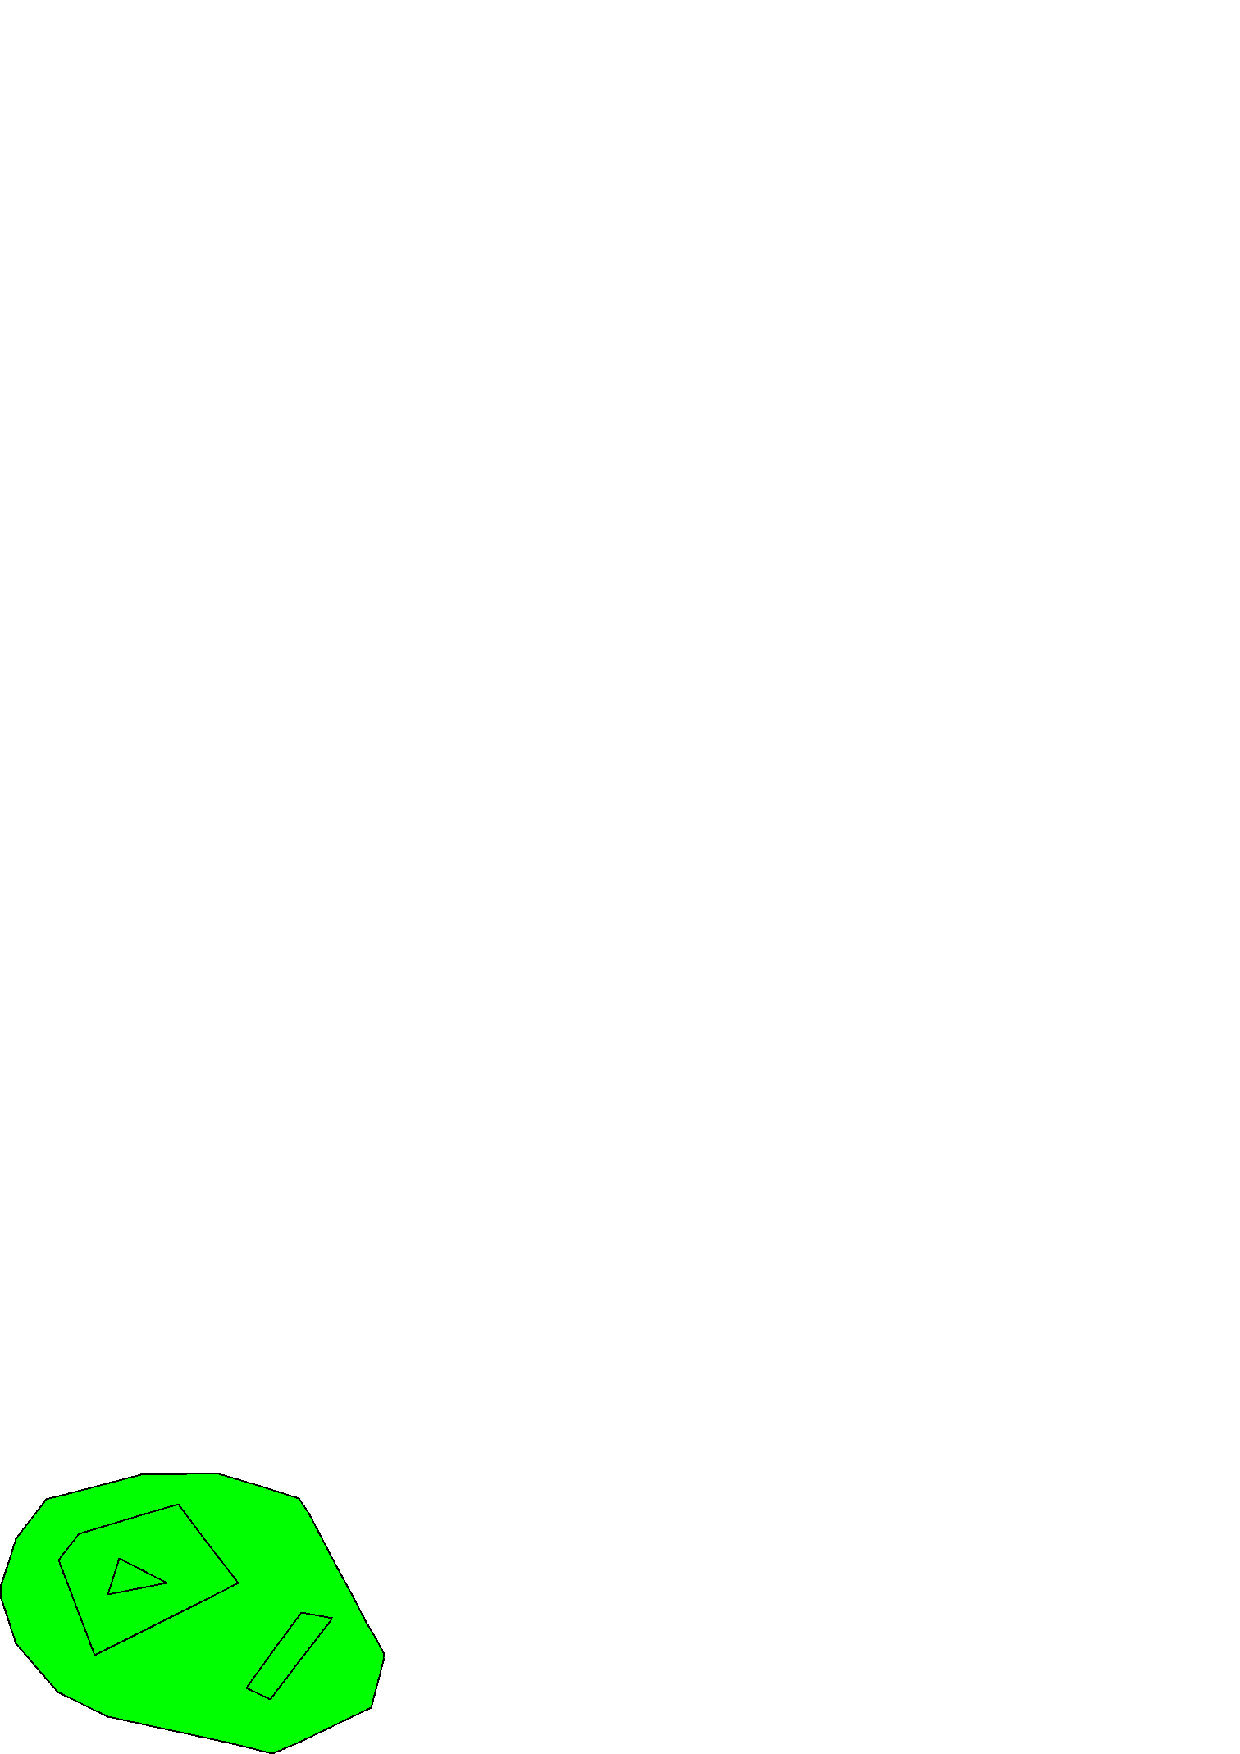
\includegraphics[width=8cm]{Mesh_2/domain}
\end{center}
\end{ccTexOnly}
\caption{A domain defined without seed points.}
\label{Domain}

\begin{ccHtmlOnly}
<center>
<img border=0 src="./domain.png"
     align=center title="A domain defined without seed points.">
</center>
\end{ccHtmlOnly}
\end{figure}

\begin{figure}[htbp]
\begin{ccTexOnly}
\begin{center}
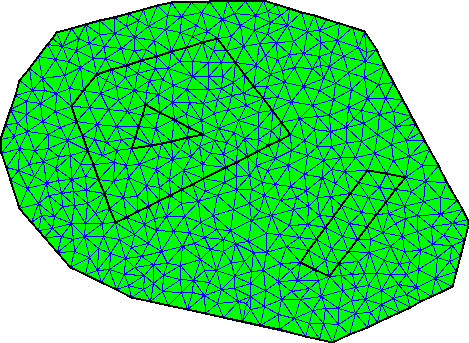
\includegraphics[width=8cm]{Mesh_2/domain-mesh}
\end{center}
\end{ccTexOnly}
\caption{A mesh of the domain defined without seed points.}
\label{Domain-mesh}

\begin{ccHtmlOnly}
<center>
<img border=0 src="./domain-mesh.png"
     align=center title="A mesh of the domain defined without seed points.">
</center>
\end{ccHtmlOnly}
\end{figure}

\begin{figure}[htbp]
\begin{ccTexOnly}
\begin{center}
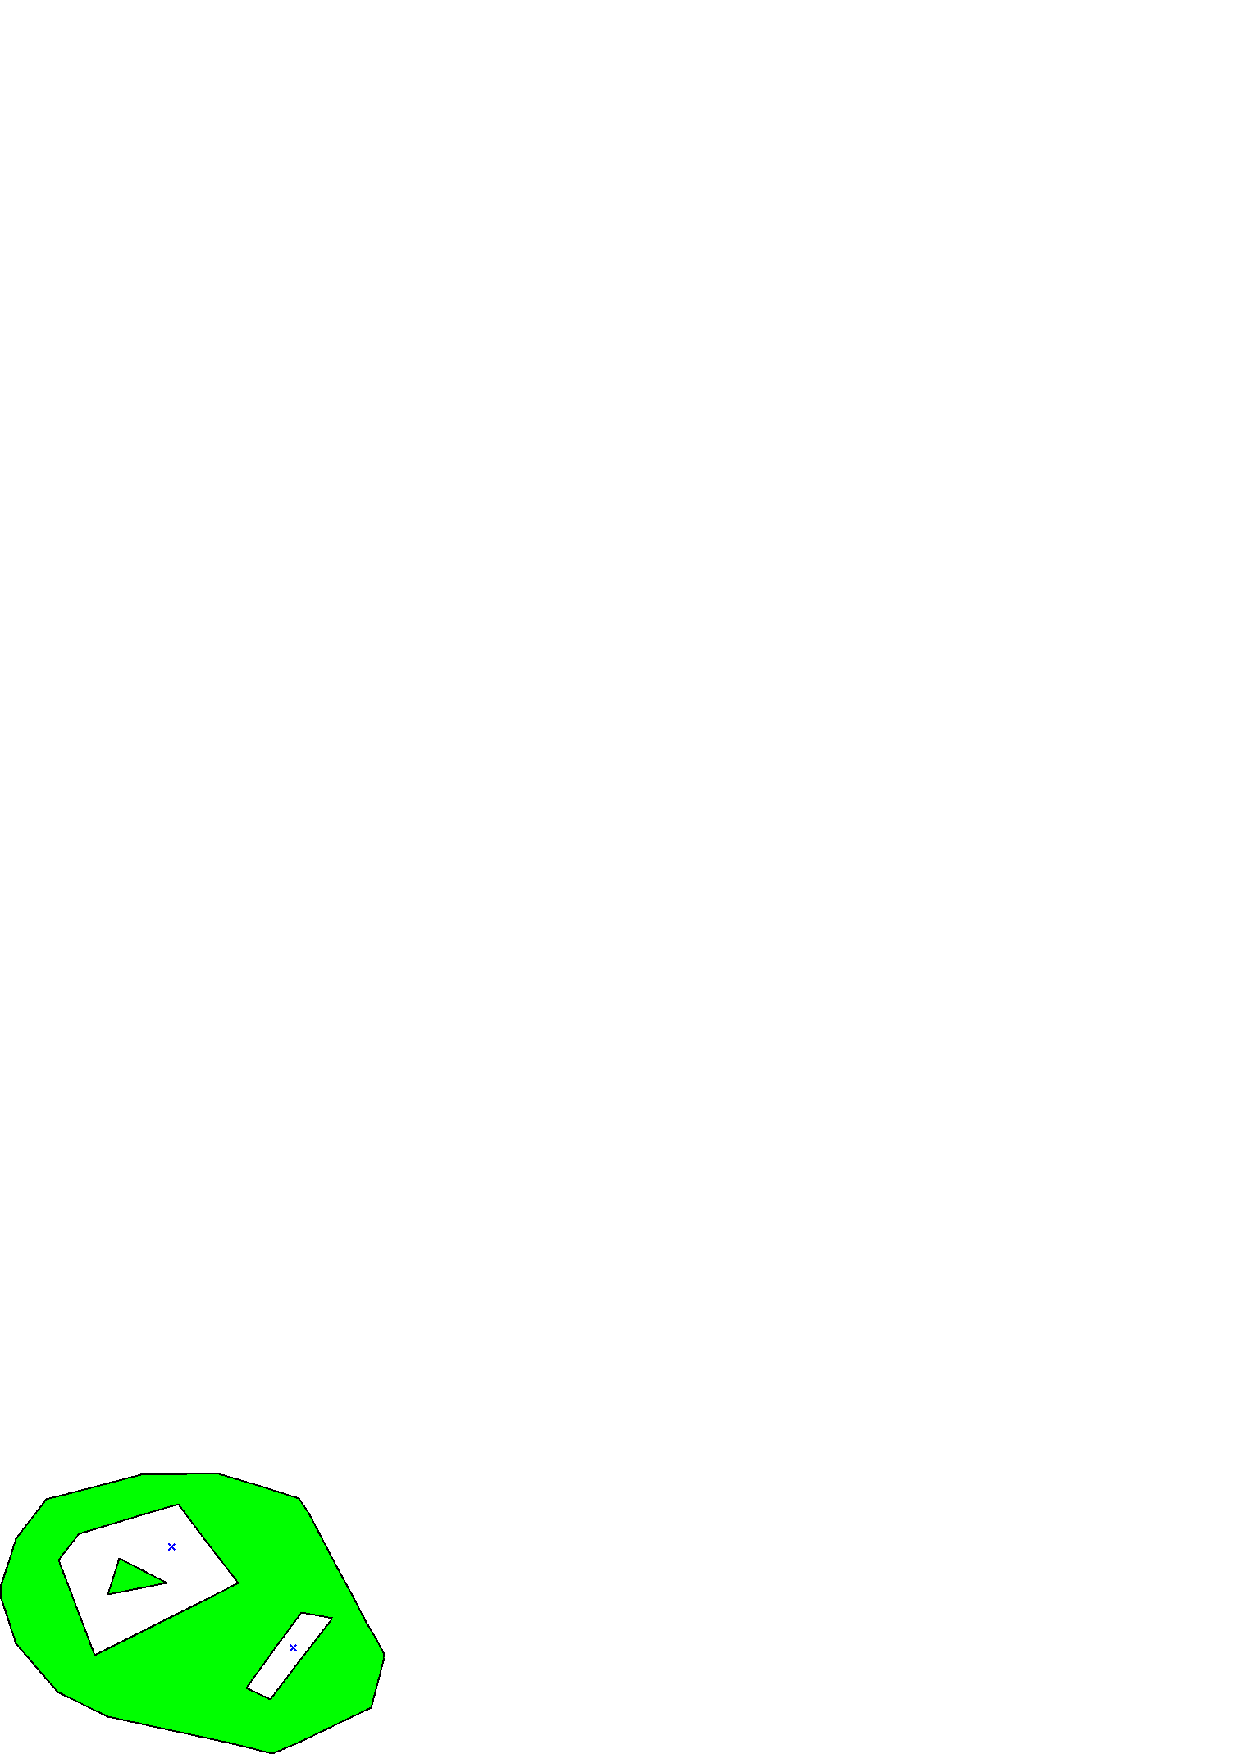
\includegraphics[width=8cm]{Mesh_2/domain-seeds}
\end{center}
\end{ccTexOnly}
\caption{A domain with two seeds points defining holes.}
\label{Domain-seeds}

\begin{ccHtmlOnly}
<center>
<img border=0 src="./domain-seeds.png"
     align=center title="A domain with two seeds points defining holes.">
</center>
\end{ccHtmlOnly}
\end{figure}

\begin{figure}[htbp]
\begin{ccTexOnly}
\begin{center}
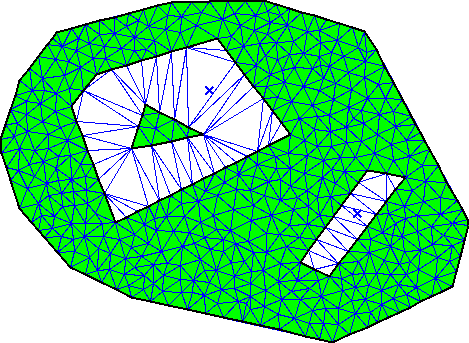
\includegraphics[width=8cm]{Mesh_2/domain-seeds-mesh}
\end{center}
\end{ccTexOnly}
\caption{A mesh of the domain with seeds defining holes.}
\label{Domain-seeds-mesh}

\begin{ccHtmlOnly}
<center>
<img border=0 src="./domain-seeds-mesh.png"
     align=center title="A mesh of the domain with seeds defining holes.">
</center>
\end{ccHtmlOnly}
\end{figure}

\subsection{Shape and Size Criteria}
\label{sec:Mesh_2_criteria}

The shape criterion on triangles is a lower bound $B$ on the ratio
between the circumradius and the shortest edge length.  Such a bound
implies a lower bound of $\arcsin{\frac{1}{2B}}$ on the minimum angle
of the triangle and an upper bound of $\pi - 2* \arcsin{\frac{1}{2B}}$
on the maximum angle.  Unfortunately, the termination of the algorithm
is guaranteed only if $B \ge \sqrt{2}$ which corresponds to a lower
bound of $20.7$~degrees on the angles.

The size criterion can be any criterion that tends to prefer small
triangles. For example, the size criterion can be an upper bound on the
length of longest edge of triangles, or an upper bound on the radius of the
circumcircle. The size bound can be varying over the domain. For example,
the size criterion could impose a small size for the triangles intersecting
a given line.

Both types of criteria are defined in an object \ccc{criteria} passed as
parameter of the meshing functions.

\subsection{The Meshing Algorithm}

The input to a meshing problem is a {\sc Pslg} and a set of seeds
describing the domain to be meshed, and a set of size and shape
criteria.  The algorithm implemented in this package starts with a
constrained Delaunay triangulation of the input {\sc Pslg} and produces a
mesh using the Delaunay refinement method. That method inserts points into
the triangulation, as far as possible from other points, and stops when the
criteria are satisfied.

If all angles between incident segments of the input {\sc Pslg}
are greater than $60$~degrees and if the bound on the
circumradius/edge ratio is greater than $\sqrt{2}$,
the algorithm is guaranteed to end up with a mesh
satisfying the size and shape criteria.

If some input angles are smaller than $60$~degrees, the algorithm will
end up with a mesh in which some triangles near small input angles
violate the criteria.  This is unavoidable since small angles formed
by input segments cannot be suppressed. Furthermore, it has been
proven (\cite{s-mgdsa-00}), that some domains with small input angles
cannot be meshed with angles even smaller than the small input angles.
Note that if the domain is a polygonal region, the resulting mesh will
satisfy size and shape criteria except for the small input angles.
In addition, the algorithm may succeed in producing meshes with a lower
angle bound greater than $20.7$~degrees, but there is no such guarantee.

\subsection{Building Meshes}
\label{sec:Mesh_2_building_meshes}

Meshes are obtained from
constrained Delaunay triangulations by calling the global function \\
\ccc{template<class CDT, class Criteria> void refine_Delaunay_mesh_2 (CDT
  &t, typename CDT::Geom_traits gt)}. \\
The template parameter \ccc{CDT} must be instantiated by a constrained
Delaunay triangulation class that is a model of the concept
\ccc{ConstrainedDelaunayTriangulation_2}. In order to override the domain,
a version of this function has two more arguments that define a sequence of
seed points.

The geometric traits class of \ccc{CDT} has to be a
model of the concept \ccc{DelaunayMeshTraits_2}.  This concept
refines the concept \ccc{ConformingDelaunayTriangulationTraits_2}
adding the geometric predicates and constructors. The template parameter
\ccc{Criteria} must be a model of \ccc{MeshingCriteria_2}. This concept
defines criteria that the triangles have to satisfy.
\cgal\ provides several models for this concept such as:
\begin{itemize}
\item \ccc{Delaunay_mesh_criteria_2<CDT>}, that defines a shape criterion
  that bounds the minimum angle of triangles, 
\item \ccc{Delaunay_mesh_size_criteria_2<CDT>}, that adds to the previous one a
  bound on the maximum edge length.
\end{itemize}

If the function \ccc{refine_Delaunay_mesh_2} is called several times on the
same triangulation with different criteria, the algorithm will rebuild used
internal data at every call. In order to avoid that, the advanced user can
use the class \ccc{Delaunay_mesher_2<CDT>}. That class provides also step
by step functions. Those functions insert one point at a time.

Any object of type \ccc{Delaunay_mesher_2<CDT>} is constructed from a
reference to a \ccc{CDT} and it has several member functions to define the
domain to be meshed and to mesh the \ccc{CDT}. See the example given below
and the reference manual for details. Note that the \ccc{CDT} should not be
externally modified during the life time of the \ccc{Delaunay_mesher_2<CDT>}
object.

\subsection{Example Using the Global Function}

The following example inserts several segments into a constrained
triangulation and then meshes it using the global function
\ccc{refine_Delaunay_mesh_2}. The size and shape criteria are the defaults
provided by the criteria class \ccc{Delaunay_mesh_criteria_2<K>}. No seeds are
given, meaning that the mesh domain covers the whole plane except for the
unbounded component.

\ccIncludeExampleCode{Mesh_2/mesh_global.C}

\subsection{Example Using the Class \protect\ccc{Delaunay_mesher_2<CDT>}}

This example uses the class \ccc{Delaunay_mesher_2<CDT>} and calls
  the \ccc{refine_mesh()} member function twice changing the size and
  shape criteria in between. In such a case, using twice the global
  function \ccc{refine_Delaunay_mesh_2} would be less efficient,
  because some internal structures needed by the algorithm would be
  built twice.

\ccIncludeExampleCode{Mesh_2/mesh_class.C}

\subsection{Example Using Seeds}

This example uses the global function \ccc{refine_Delaunay_mesh_2} but
defines a domain by using one seed. The size and shape criteria are the
defaults provided by the criteria class \ccc{Delaunay_mesh_criteria_2<K>}.

\ccIncludeExampleCode{Mesh_2/mesh_with_seeds.C}

%%% For emacs/AucTeX:
%%% Local Variables: ***
%%% mode:latex ***
%%% TeX-master: "../Mesh_2.tex"  ***
%%% End: ***
